\chapter{Diferenciación e integración numérica}

\section{Fórmula de diferencia progresiva y regresiva}
La definición de la derivada de una función $f(x)$ en un punto $x$ es
\begin{equation}
	f'(x) = \lim_{h\rightarrow 0} \dfrac{f(x+h)-f(x)}{h}
\end{equation}
la cual se puede interpretar geométricamente como la pendiente de la recta tangente al punto dado por $x$. 

\subsection{Diferencia progresiva}
De manera alternativa, se puede obtener una aproximación a la derivada a través de una recta secante 
a la función. Esto se puede ver en la figura \ref{fig:derivadaProgresiva}.

\begin{figure}[ht]
	\centering
	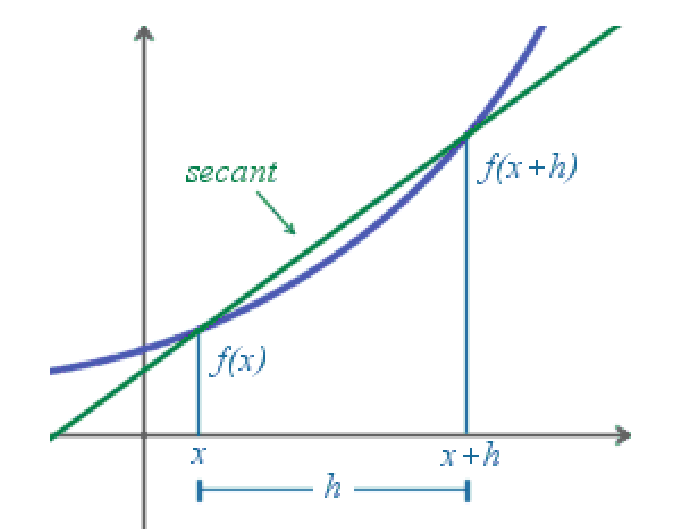
\includegraphics[scale=0.35]{img/derivadaProgresiva.png}
	\caption{Derivada progresiva}
	\label{fig:derivadaProgresiva}
\end{figure}

Calculando la pendiente de la recta secante de la figura \ref{fig:derivadaProgresiva} se obtiene una aproximación a la derivada.
\begin{align}
	m &= \dfrac{f(x+h)-f(x)}{x+h-x}\nonumber\\
		&= \dfrac{f(x+h)-f(x)}{h}\nonumber\\
	f'(x) &= \dfrac{f(x+h)-f(x)}{h}
	\label{eq:derivadaProgresiva1}
\end{align}

La expresión (\ref{eq:derivadaProgresiva1}) es una aproximación a la derivada de la función $f(x)$ 
siempre y cuando el valor de $h$ sea pequeño. Sin embargo, para una aproximación más exacta a la primera derivada se puede 
utilizar una serie de Taylor (\ref{eq:serieTaylor}).
\begin{align}
	f(x) &= \sum_{n=0}^\infty \dfrac{f^{(n)}(a)}{n!}(x-a)^n\nonumber\\
		&= f(a) + \dfrac{f'(a)}{1!}(x-a) + \dfrac{f''(a)}{2!}(x-a)^2 + \dfrac{f^{(3)}(a)}{3!}(x-a)^3 + \cdots + \dfrac{f^{(n)}(a)}{n!}(x-a)^n
	\label{eq:serieTaylor}
\end{align}


Desarrollando la serie para $f(x)$ centrada en $a=x$ y para $x=x+h$.
\begin{align*}
	f(x+h) &= f(x) + \dfrac{f'(x)}{1!}(x+h-x) + \dfrac{f''(x)}{2!}(x+h-x)^2 + \cdots + \dfrac{f^{(n)}(x)}{n!}(x+h-x)^n\\
		&= f(x) + f'(x)\cdot h + \dfrac{f''(x)}{2!}\cdot h^2 + \cdots + \dfrac{f^{(n)}(x)}{n!}\cdot h^n\\
\end{align*}
Dado que sólo nos interesa la primera derivada, se toman los primeros tres términos de la serie.
\begin{align*}
	f(x+h) &\approx f(x) + f'(x)\cdot h + \dfrac{f''(x)}{2!}\cdot h^2
\end{align*}
Despejando $f'(x)$ se obtiene la expresión (\ref{eq:derivadaProgresiva2})
\begin{definitionT}
	\begin{align}
		f'(x) &\approx \dfrac{f(x+h)-f(x)}{h} - \dfrac{f''(x)}{2!}\cdot h.
		\label{eq:derivadaProgresiva2}
	\end{align}
\end{definitionT}

\subsection{Diferencia regresiva}
Otra alternativa es aproximar la derivada de nueva cuenta con una recta secante a la función. Vease la figura \ref{fig:derivadaRegresiva}.
\begin{figure}[ht]
	\centering
	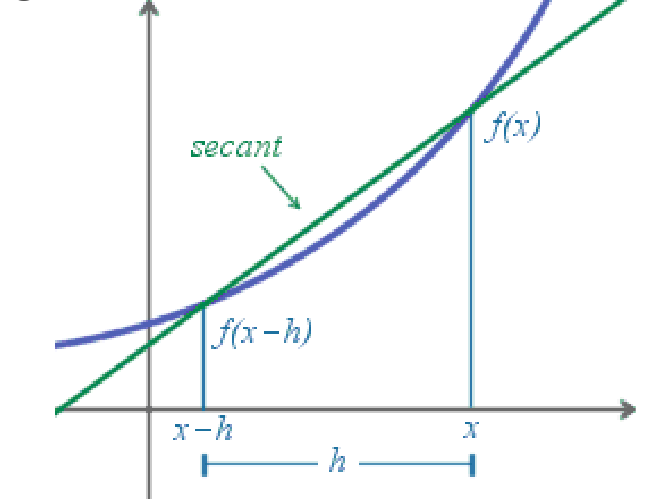
\includegraphics[scale=0.35]{img/derivadaRegresiva.png}
	\caption{Derivada regresiva}
	\label{fig:derivadaRegresiva}
\end{figure}

La diferencia sustancial en esta variante del procedimiento es que el valor diferencial $h$ se resta, en lugar de sumarse tal como el caso
anterior. Esto implica que el punto para formar la recta secante será anterior a $x$.

Calculando la pendiente de la recta secante para esta alternativa de la figura \ref{fig:derivadaRegresiva} se obtiene otra aproximación 
a la derivada.
\begin{align}
	m &= \dfrac{f(x)-f(x-h)}{x-(x-h)}\nonumber\\
	f'(x) &= \dfrac{f(x)-f(x-h)}{h}
	\label{eq:derivadaRegresiva1}
\end{align}
De nueva cuenta la expresión (\ref{eq:derivadaRegresiva1}) es una aproximación a la derivada de la función $f(x)$ 
siempre y cuando el valor de $h$ sea pequeño. Se desarrolla ahora la serie de Taylor para $f(x)$ centrada en $a=x-h$ y para $x=x$.
\begin{align*}
	f(x-h) &= f(x) + \dfrac{f'(x)}{1!}(x-h-x) + \dfrac{f''(x)}{2!}(x-h-x)^2 + \cdots + \dfrac{f^{(n)}(x)}{n!}(x-h-x)^n\\
		&= f(x) - f'(x)\cdot h + \dfrac{f''(x)}{2!}\cdot h^2 + \cdots + (-1)^n\cdot\dfrac{f^{(n)}(x)}{n!}\cdot h^n\\
\end{align*}
Dado que sólo nos interesa la primera derivada, se toman los primeros tres términos de la serie.
\begin{align*}
	f(x-h) &\approx f(x) - f'(x)\cdot h + \dfrac{f''(x)}{2!}\cdot h^2
\end{align*}
Despejando $f'(x)$  se obtiene la expresión (\ref{eq:derivadaRegresiva2})
\begin{definitionT}[Derivada Regresiva]
	\begin{equation}
		f'(x) \approx \dfrac{f(x)-f(x-h)}{h} + \dfrac{f''(x)}{2!}\cdot h.
	\label{eq:derivadaRegresiva2}
	\end{equation}
\end{definitionT}

\begin{exerciseT}{\rm
Utilice la derivada progresiva y regresiva para encontrar una aproximación a la derivada de la función $f(x) = xe^x$ en $x=2$. 
Compare los resultados obtenidos por ambos métodos.

\subsection*{Planteamiento}
Para este ejercicio se utilizará $h=0.1$. 

\subsection*{Desarrollo}

Derivación Progresiva
\begin{align*}
	f'(2) &\approx \dfrac{f(2+0.1)-f(2)}{0.1} = \dfrac{f(2.1)-f(2)}{0.1} \\
		&\approx \dfrac{2.1e^{2.1}-2e^2}{0.1}\\
		&\approx 23.7084
\end{align*}

Derivación Regresiva
\begin{align*}
	f'(2) &\approx \dfrac{f(2)-f(2-0.1)}{0.1} = \dfrac{f(2)-f(1.9)}{0.1} \\
		&\approx \dfrac{2e^2 - 1.9e^{1.9}}{0.1}\\
		&\approx 20.7491
\end{align*}
La figura \ref{fig:derivada01} muestra una comparación de las rectas obtenidas por estos cálculos, estas rectas
secante son aproximaciones a la tangente, que a su vez es la derivada de la función para $x=2$.
\begin{figure}[H]
	\centering
	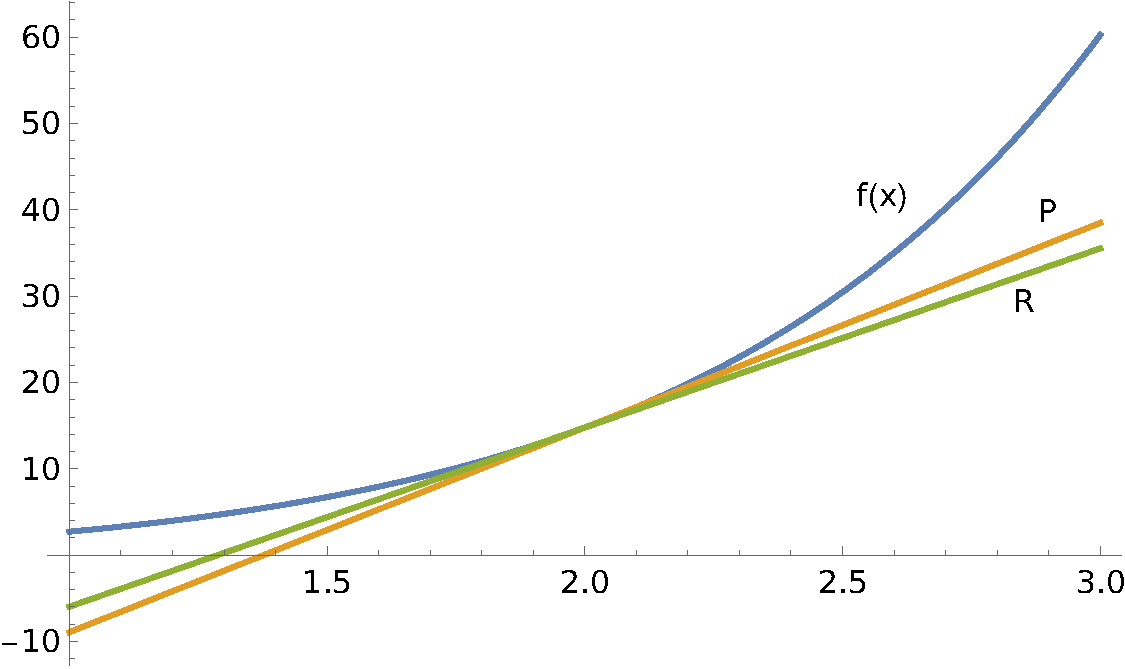
\includegraphics[scale=0.5]{img/Derivada01.pdf}
	\caption{Comparación de las primeras aproximaciones del Ejemplo \ref{ex:derivada01}}
	\label{fig:derivada01}
\end{figure}
La recta naranja (marcada con la letra P) corresponde a la obtenida por la derivación progresiva, mientras que la 
recta verde (marcada con la letra R) corresponde a la obtenida por derivación regresiva.

Es notorio que para obtener un mejor resultado en las aproximaciones se debe utilizar un valor más pequeño para $h$.
Gráficamente observaríamos que las rectas secantes se aproximan cada vez más a la tangente. La tabla \ref{table:derivada01} 
muestra los cálculos para diversos valores de $h$.

\begin{table}[H]
	\centering
	\begin{tabular}{ccc}
		\toprule
		h & D. Progresiva & D. Regresiva \\
		\midrule
		0.1 & 23.7084 & 20.7491 \\
		0.05 & 22.9217 & 21.4434 \\
		0.01 & 22.3156 & 22.02 \\
		0.005 & 22.2412 & 22.0934 \\
		0.001 & 22.182 & 22.1524 \\
		0.0001 & 22.1686 & 22.1657 \\
		0.00001 & 22.1673 & 22.167\\
		\bottomrule
	\end{tabular}
	\label{table:derivada01}
	\caption{Resultados del Ejercicio \ref{ex:derivada01}}
\end{table}
\label{ex:derivada01}
}\end{exerciseT}

\section{Fórmula de tres puntos}
\label{section:d3p}
Una estrategia distinta para obtener aproximaciones a la derivada de una función consiste en utilizar la interpolación para ello.
La idea se basa en el hecho de que un polinomio es continuo y derivable para todos los números reales. Como una ventaja adicional, 
el polinomio es fácilmente derivable. 

De esta forma la estrategia consiste en construir un polinomio de interpolación que aproxime 
a la función que se desea derivar, ahora se deriva el polinomio y se evalúa en el punto que se desea aproximar. De acuerdo al grado
del polinomio que se haya construido, la aproximación del resultado con la derivada será mejor. En términos generales se puede decir
que \textit{a mayor grado del polinomio mejor la aproximación a la derivada}.

Para la construcción del polinomio se utiliza la interpolación de Lagrange de la ecuación (\ref{eq:polinomioLagrange}). Supongamos 
que $\{x_0,x_1,\dots,x_n\}$ son $(n+1)$ números distintos en algún intervalo $I$ y que $f\in C^{n+1}(I)$. Entonces:
\[ f(x) = \sum_{k=0}^n f(x_k)L_{n,k}(x) \]
Al derivar esta expresión y evaluar $x=x_j$ se obtiene
\begin{equation}
	f'(x_j) = \sum_{k=0}^n f(x_k)L'_{n,k}(x_j)
	\label{eq:formula(n+1)Puntos} 
\end{equation}

que recibe el nombre de fórmula de $(n+1)$ puntos para aproximar $f'(x_j)$ donde $x_j$ es el valor en el que se evalúa la derivada.

En términos generales, la utilización de más puntos de evaluación en la ecuación (\ref{eq:formula(n+1)Puntos}) produce una mayor 
exactitud, aunque esto puede no ser conveniente dada la cantidad de evaluaciones funcionales y el aumento en el error de redondeo. 
Por esta razón es que se limita a formulas de tres y cinco puntos de evaluación. 

Para los tres puntos el polinomio de interpolación de Lagrange que corresponde es de segundo grado
\[ f(x) = f(x_0)L_0(x) + f(x_1)L_1(x) + f(x_2)L_2(x) \]
y su derivada es
\[ f'(x) = f(x_0)L_0'(x) + f(x_1)L_1'(x) + f(x_2)L_2'(x).\]
De esta forma, el primer término de Lagrange es
\[ L_0(x) = \dfrac{(x-x_1)(x-x_2)}{(x_0-x_1)(x_0-x_2)} \]
y su derivada con respecto a $x$ es
\[ L'_0(x) = \dfrac{2x-x_1-x_2}{(x_0-x_1)(x_0-x_2)}. \]
Para los términos de Lagrange $L_1$ y $L_2$ el resultado es muy similar, por lo que son 
\[ L'_1(x) = \dfrac{2x-x_0-x_2}{(x_1-x_0)(x_1-x_2)} \]
y 
\[ L'_2(x) = \dfrac{2x-x_0-x_1}{(x_2-x_0)(x_2-x_1)}. \]
Ahora sustituyendo la derivada de los términos de Lagrange en la ecuación \ref{eq:formula(n+1)Puntos} queda,
\begin{equation}
	f'(x_j) = f(x_0)\left[\dfrac{2x_j - x_1 - x_2}{(x_0-x_1)(x_0-x_2)}\right] + 
	f(x_1)\left[\dfrac{2x_j - x_0 - x_2}{(x_1-x_0)(x_1-x_2)}\right] 
	+ f(x_2)\left[{2x_j - x_0 - x_1\over (x_2-x_0)(x_2-x_1)}\right].
	\label{eq:formulaDerivadaTresPuntos}
\end{equation}
La ecuación (\ref{eq:formulaDerivadaTresPuntos}) es una aproximación a la derivada de $f$ evaluada en $x_j$ para tres puntos:
$x_0$, $x_1$ y $x_2$.

Ahora, si se distribuyen los puntos de forma equidistante, esto es 
\begin{align*}
	\mbox{Sea }& h\in\mathbb{R} \wedge h\not=0 \\
	x_j &= x_0\\
	x_1 &= x_0 + h \\ 
	x_2 &= x_1 + h = x_0+2h,
\end{align*}
entonces la ecuación (\ref{eq:formulaDerivadaTresPuntos}) se reduce a la expresión (\ref{eq:d3ppe}).

\begin{definitionT}[Fórmula de tres puntos - punto extremo]
	\begin{equation}
		f'(x_0) = \dfrac{1}{2h}\left[-3f(x_0)+4f(x_0+h)-f(x_0+2h)\right]
		\label{eq:d3ppe}
	\end{equation}
\end{definitionT}

Ahora, utilizando nuevamente la expresión (\ref{eq:formulaDerivadaTresPuntos}) con los tres puntos $x_0$, $x_1$ y $x_2$ 
pero acomodandolos de manera equidistante pero con $x_0$ al centro, esto es:
\begin{align*}
	\mbox{Sea }& h\in\mathbb{R} \wedge h\not=0 \\
	x_j &= x_0\\
	x_1 &= x_0 - h \\ 
	x_2 &= x_0 + h,
\end{align*}
entonces la ecuación (\ref{eq:formulaDerivadaTresPuntos}) se reduce a la expresión (\ref{eq:d3ppm}).

\begin{definitionT}[Fórmula de tres puntos - punto medio]
	\begin{equation}
		f'(x_0) = \frac{1}{2h}\left[f(x_0+h) - f(x_0-h)\right] 
		\label{eq:d3ppm}
	\end{equation}
\end{definitionT}

\section{Fórmula de cinco puntos}
Los métodos presentados en las ecuaciones (\ref{eq:d3ppe}) y (\ref{eq:d3ppm}) reciben el nombre de \textbf{fórmulas de tres 
puntos}. Así mismo, existen las llamadas \textbf{fórmulas de cinco puntos} que implican la evaluación de la función en 
dos puntos más, pero cuyo término de error tiene la forma $O(h^4)$. 

Retomando la estrategia utilizada para las fórmulas de los tres puntos, en la expresión (\ref{eq:formula(n+1)Puntos})
pero ahora se consideran cinco puntos. La expresión se reduce a
\[ f(x) = f(x_0)L_0(x) + f(x_1)L_1(x) + f(x_2)L_2(x) + f(x_3)L_3(x) + f(x_4)L_4(x) \]
y su derivada es
\begin{equation}
	f'(x_j) = f(x_0)L_0'(x) + f(x_1)L_1'(x) + f(x_2)L_2'(x) + f(x_3)L'_3(x) + f(x_4)L'_4(x).
	\label{eq:formula5puntos}
\end{equation}
De esta forma, el primer término de Lagrange es
\[ L_0(x) = \dfrac{(x-x_1)(x-x_2)(x-x_3)(x-x_4)}{(x_0-x_1)(x_0-x_2)(x_0-x_3)(x_0-x_4)} \]
y su derivada con respecto a $x$ es
\[ 
	L'_0(x) = \dfrac{(x-x_1)(x-x_2)(x-x_3)+(x-x_1)(x-x_2)(x-x_4)+(x-x_1)(x-x_3)(x-x_4)+(x-x_2)(x-x_3)(x-x_4)}
	{(x_0-x_1)(x_0-x_2)(x_0-x_3)(x_0-x_4)}. 
\]
Para los términos de Lagrange  restantes $L'_1$, $L'_2$, $L'_3$ y $L'_4$ el resultado es muy similar. Sustituyendo todos ellos
en la expresión (\ref{eq:formula5puntos}), reducir los términos se obtiene una expresión semejante a (\ref{eq:formulaDerivadaTresPuntos}).

Ahora, si se distribuyen los 5 puntos $x_0$, $x_1$, $x_2$, $x_3$ y $x_4$ de forma equidistante, y el valor $x_0$ encontrándose
en el extremo izquierdo, esto es:
\begin{align*}
	\mbox{Sea }& h\in\mathbb{R} \wedge h\not=0 \\
	x_j &= x_0\\
	x_1 &= x_0 + h \\ 
	x_2 &= x_0 + 2h \\
	x_3 &= x_0 + 3h \\
	x_4 &= x_0 + 4h
\end{align*}
entonces se reduce a la expresión (\ref{eq:d5ppe}).

\begin{definitionT}[Fórmula de cinco puntos - punto extremo]
	\begin{equation}
		f'(x_0) = \frac{1}{12h}\left[-25f(x_0) + 48f(x_0+h) - 36f(x_0+2h) + 16f(x_0+3h) - 3f(x_0+4h)\right]
		\label{eq:d5ppe}
	\end{equation}
\end{definitionT}

Si por otro lado se distribuyen los 5 puntos $x_0$, $x_1$, $x_2$, $x_3$ y $x_4$ de forma equidistante, y el valor $x_0$ encontrándose
en el centro, esto es:
\begin{align*}
	\mbox{Sea }& h\in\mathbb{R} \wedge h\not=0 \\
	x_j &= x_0\\
	x_1 &= x_0 - h \\ 
	x_2 &= x_0 - 2h \\
	x_3 &= x_0 + h \\
	x_4 &= x_0 + 2h
\end{align*}
entonces se reduce a la expresión (\ref{eq:d5ppm}).

\begin{definitionT}[Fórmula de cinco puntos - punto medio]
	\begin{equation}
		f'(x_0) = \frac{1}{12h}\left[f(x_0-2h) - 8f(x_0-h) + 8f(x_0+h) - f(x_0+2h) \right]
		\label{eq:d5ppm}
	\end{equation}
\end{definitionT}

\section{Fórmula de 3 puntos para la segunda derivada}
Si se retoma el procedimiento de la sección \ref{section:d3p} y en particular la expresión (\ref{eq:formula(n+1)Puntos}), sólo
que en esta ocasión se deriva nuevamente la expresión para obtener una segunda derivada del polinomio $f(x)$ dado por la serie 
de Taylor. Esto es:
\begin{equation}
	f''(x_j) = \sum_{k=0}^n f(x_k)L''_{n,k}(x_j)
	\label{eq:formula2d(n+1)Puntos} 
\end{equation}
Esta expresión (\ref{eq:formula2d(n+1)Puntos}) requiere a su vez de la segunda derivada de $L_0$, $L_1$ y $L_2$. Derivando estos
términos y sustituyendo se obtendría una expresión semejante a (\ref{eq:formulaDerivadaTresPuntos}). Ahora distribuyendo de 
forma equidistante los valores $x_0$, $x_1$ y $x_2$, con el valor $x_0$ en el centro, esto es:
\begin{align*}
	\mbox{Sea }& h\in\mathbb{R} \wedge h\not=0 \\
	x_j &= x_0\\
	x_1 &= x_0 - h \\ 
	x_2 &= x_0 + h,
\end{align*}
entonces la ecuación (\ref{eq:formula2d(n+1)Puntos}) se reduce a la expresión (\ref{eq:2d3ppm}).
\begin{definitionT}[Fórmula segunda derivada tres puntos - punto medio]
	\begin{equation}
		f''(x_0) = \frac{1}{h^2}\left[f(x_0-h) - 2f(x_0) + f(x_0+h)\right] 
		\label{eq:2d3ppm}
	\end{equation}
\end{definitionT}


\begin{exerciseT}
	Dada la función $f(x) = xe^x$, 
		\begin{enumerate}[a)]
			\item Utilice las fórmulas de los 3 y 5 puntos para encontrar aproximaciones a la primera derivada de 
				la función $f(x)$ en $x=2$. 
			\item ¿Qué fórmula permite encontrar un mejor resultado?, ¿porque?
			\item Utilice también la fórmula de los 3 puntos para obtener una aproximación a la segunda derivada de $f(x)$ en $x=2$.
		\end{enumerate}	
	\subsection*{Desarrollo}
	Dado que no se indica el valor de $h$ se asume que tiene el valor de $0.1$.\\
	a) Primera derivada
	\begin{align*}
		&\mbox{Fórmula de 3 puntos - punto extremo}\\
		x_0 &= 2\\
		h &= 0.1\\
		f'(2) &= \dfrac{1}{2(0.1)}\left[-3f(2) + 4f(2.1) - f(2.2)\right]\\
			&= 22.03230486614652
	\end{align*}
	\begin{align*}
		&\mbox{Fórmula de 3 puntos - punto medio}\\
		x_0 &= 2\\
		h &= 0.1\\
		f'(2) &= \dfrac{1}{2(0.1)}\left[f(2.1)-f(1.9)\right]\\
			&= 22.228786880307297
	\end{align*}
	\begin{align*}
		&\mbox{Fórmula de 5 puntos - punto extremo}\\
		x_0 &= 2\\
		h &= 0.1\\
		f'(2) &= \dfrac{1}{12(0.1)}\left[-25f(2)+48f(2.1)-36f(2.2)+16f(2.3)-3f(2.4)\right]\\
			&= 22.165914568055193
	\end{align*}
	\begin{align*}
		&\mbox{Fórmula de 5 puntos - punto medio}\\
		x_0 &= 2\\
		h &= 0.1\\
		f'(2) &= \dfrac{1}{12(0.1)}\left[f(1.8)-8f(1.9)+8f(2.1)-f(2.2)\right]\\
			&= 22.166995621399924
	\end{align*}
	b) Las fórmulas de los 5 puntos dan mejores resultados que las de 3 puntos en términos generales. Para 
	mejorar aún más la aproximación sería conveniente hacer más pequeño el valor de $h$.\\
	c) Segunda derivada
	\begin{align*}
		&\mbox{Fórmula de 3 puntos - punto medio}\\
		x_0 &= 2\\
		h &= 0.1\\
		f''(2) &= \dfrac{1}{(0.1)^2}\left[f(1.9)-2f(2)+f(2.1)\right]\\
			&= 29.593186100007426
	\end{align*}
\end{exerciseT}

\section{Integración numérica: Método del trapecio}
Para deducir la regla del trapecio para aproximar la integral definida \[\int_a^b f(x)dx, \] sea $x_0=a$, $x_1=b$, $h=b-a$  se puede
utilizar la misma estrategía que en la derivación numérica. Esto es, se construye un polinomio de interpolación $P(x)$ para $f(x)$ 
y finalmente este es el que se integra. De esta forma, se utiliza un polinomio lineal de Lagrange para los valores $x_0=a$ y $x_1=b$,
esto es: 
\[ P_1(x) = \dfrac{x-x_1}{x_0-x_1}f(x_0) + \dfrac{x-x_0}{x_1-x_0}f(x_1).\]
Luego se integra $P_1$,
\begin{align}
  \int_a^b f(x)dx = \int_{x_0}^{x_1} \left[ \dfrac{x-x_1}{x_0-x_1}f(x_0) + \dfrac{x-x_0}{x_1-x_0}f(x_1)  \right]dx.
  \label{eq:trapecio1}
\end{align}
Resolviendo la integral de la ecuación (\ref{eq:trapecio1})
\begin{align*}
  \int_a^b f(x)dx &= \left[ {(x-x_1)^2\over 2(x_0-x_1) }f(x_0) + {(x-x_0)^2\over 2(x_1-x_0)}f(x_1) \right]_{x_0}^{x_1} \\
	&= \left[ \dfrac{x_1-x_0}{2}f(x_1) - \dfrac{x_0-x_1}{2}f(x_0) \right] \\
  	&= \frac{x_1-x_0}{2}\left[f(x_0) + f(x_1)\right].
\end{align*}

Retomando la notación $h=x_1-x_0$ se tiene:
\subsection*{}
\begin{definitionT}[Regla del Trapecio]
	\begin{equation}
		\int_a^b f(x)dx = \dfrac{h}{2}\left[f(x_0) + f(x_1)\right].
		\label{eq:reglaTrapecio} 
	\end{equation}	
\end{definitionT}

La expresión (\ref{eq:reglaTrapecio}) se llama \textbf{regla del trapecio} que justamente utiliza un trapecio para realizar
la aproximación al área bajo la curva de $f(x)$ desde $x=a$ hasta $x=b$. Esto se muestra en la figura \ref{fig:reglaTrapecio}.
\begin{figure}[H]
	\centering
	\includegraphics[scale=0.15]{../img/reglaTrapecio.jpg}
  	\caption{Regla del Trapecio}
  	\label{fig:reglaTrapecio}
\end{figure}


\section{Integración numérica: Método de Simpson}
Para este método se utiliza la misma estrategia que el método del trapecio. Ahora para el método de Simpson se integra el polinomio 
de Lagrange de segundo grado. Por esta razón es que se requieren de tres valores $x_0$, $x_1$ y $x_2$. Los puntos se encuentran
igualmente distanciados y ubicados en los límites de integración $[a,b]$, esto es:
\begin{align*}
	h &= \dfrac{b-a}{2} \\
	x_0 &= a \\
	x_1 &= x_0+h \\
	x_2 &= b 
\end{align*}
Esto se puede apreciar en la figura \ref{fig:reglaSimpson}.

\begin{figure}[H]
  \centering
  \includegraphics[scale=0.15]{../img/reglaSimpson.jpg}
  \caption{Regla de Simpson}
  \label{fig:reglaSimpson}
\end{figure}
El polinomio de Lagrange para estos puntos es:
\begin{align*}
	P_2(x) &= \dfrac{(x-x_1)(x-x_2)}{(x_0-x_1)(x_0-x_2)}f(x_0) +  \dfrac{(x-x_0)(x-x_2)}{(x_1-x_0)(x_1-x_2)}f(x_1) 
		\dfrac{(x-x_0)(x-x_1)}{(x_2-x_0)(x_2-x_1)}f(x_2).
\end{align*}

Este polinomio se integra en el intervalo $[x_0, x_2]$:
\begin{align*}
	\int_a^b f(x)dx = \int_{x_0}^{x_2} \left[ \dfrac{(x-x_1)(x-x_2)}{(x_0-x_1)(x_0-x_2)}f(x_0) +  
	\dfrac{(x-x_0)(x-x_2)}{(x_1-x_0)(x_1-x_2)}f(x_1) \dfrac{(x-x_0)(x-x_1)}{(x_2-x_0)(x_2-x_1)}f(x_2) \right]dx
\end{align*}

Resolviendo la integral, evaluando y simplificando términos se obtiene la expresión (\ref{eq:reglaSimpson}).

\begin{definitionT}[Regla de Simpson]
	\begin{equation}
		\int_{x_0}^{x_2} f(x)dx = \dfrac{h}{3}\left[f(x_0) + 4f(x_1) + f(x_2)\right]
		\label{eq:reglaSimpson}
	  \end{equation}
\end{definitionT}

\begin{exerciseT}
	Utilice las reglas del trapecio y Simpson para encontrar aproximaciones a la integral dada.
	\[ A = \int_0^{\pi/2} \sin xdx\]
	\begin{enumerate}[a)]
		\item Regla del trapecio
			\begin{align*}
				x_0 &= 0\\
				x_1 &= \dfrac{\pi}{2}\\
				h &= \dfrac{\pi}{2}-0 = \dfrac{\pi}{2}\\
				A &= \dfrac{\pi/2}{2}\left[\sin 0 + \sin\frac{\pi}{2}\right] = \dfrac{\pi}{4}\sin\dfrac{\pi}{2} = 0.785398 u^2
			\end{align*}
		\item Regla de Simpson
			\begin{align*}
				x_0 &= 0 \\
				x_2 &= \dfrac{\pi}{2}\\
				h &= \dfrac{\frac{\pi}{2}-0}{2} = \dfrac{\pi}{4}\\
				x_1 &= 0 + \dfrac{\pi}{4} = \dfrac{\pi}{4}\\
				A &= \dfrac{\frac{\pi}{4}}{3}\left[\sin 0 + 4\sin \frac{\pi}{4} + \sin \frac{\pi}{2} \right] 
					= \dfrac{\pi}{12}\left[4\sin \frac{\pi}{4} + \sin \frac{\pi}{2} \right] = 1.002279 u^2
			\end{align*}
	\end{enumerate}
\end{exerciseT}

\section{Integración numérica: Integración de Romberg}
La integración de Romberg requiere de la realización de un proceso de extrapolación. Para que la extrapolación obtenga  
buenos resultados, el fenómeno que se estudia debe ser predecible en cierto grado, es decir que siga un patrón definido. 
Ese fenómeno en el caso de la integración se trata del error en la aproximación (dado por la regla del trapecio), el cuál tiene en 
efecto un patrón predecible. Por esta razón, la extrapolación resulta muy adecuada para la aproximación a una integral definida.

La estrategia a seguir es la siguiente, partimos de aproximaciones iniciales y a través de la extrapolación se mejorarán dramáticamente.
Las aproximaciones iniciales podrían ser las obtenidas por la regla del trapecio, pero utilizar mejores valores iniciales mejora
los resultados obtenidos por la extrapolación. Por esa razón es que se opta por utilizar la regla compuesta del trapecio 
descrita por la expresión (\ref{eq:reglaCompuestaTrapecio}).


\begin{definitionT}[Regla compuesta del trapecio]
	Si $h=\frac{b-a}{n}$ y $x_j = a+j\cdot h$ entonces
	\begin{align}
		\int_a^b f(x)dx &= \dfrac{h}{2}\left[f(a) + 2\sum_{j=1}^{n-1} f(x_j) + f(b) \right] - \dfrac{b-a}{12}h^2f''(\mu),
		\label{eq:reglaCompuestaTrapecio}
	\end{align}	
	La regla del trapecio tiene un error de truncamiento de orden $O(h^2)$.
\end{definitionT}

Para encontrar las aproximaciones iniciales orden $O(h^2)$ de la integral $\int_a^b f(x)dx$ se usa la regla compuesta del trapecio 
(\ref{eq:reglaCompuestaTrapecio}) con $n=1,2,4,8,16,\dots$, y se dichas aproximaciones se denotan $R_{1,1}$, $R_{2,1}$, $R_{3,1}$, 
$R_{4,1}$, $R_{5,1}$, \dots respectivamente. 

Ahora ya se puede aplicar la extrapolación para obtener las aproximaciones orden $O(h^4): R_{2,2}, R_{3,2}, R_{4,2}$, $\dots$ mediante:
\begin{align*}
	R_{k,2} = R_{k,1} + \dfrac{1}{3}\left(R_{k,1} - R_{k-1,1} \right), \mbox{ para } k=2,3,\dots
\end{align*}
Luego las aproximaciones orden $O(h^6): R_{3,3}, R_{4,3}, R_{5,3}$, $\dots$ mediante:
\begin{align*}
	R_{k,3} = R_{k,2} + \dfrac{1}{15}\left(R_{k,2} - R_{k-1,2} \right), \mbox{ para } k=3,4,\dots.
\end{align*}
En términos generales, para obtener las aproximaciones orden $O(h^{2j})$ conociendo las aproximaciones $R_{k,j-1}$ se tiene:
\begin{align}
	R_{k,j} = R_{k,j-1} + \dfrac{1}{4^{j-1}-1}\left(R_{k,j-1} - R_{k-1,j-1} \right), \mbox{ para } k=j,j+1,\dots.
	\label{eq:extrapolacionRomberg}
\end{align}

El algoritmo \ref{algo:Romberg} muestra el método de la integración de Romberg.
\begin{algorithm}[ht]
  	\SetKwInOut{Input}{input}
  	\SetKwInOut{Output}{output}
  	\SetKwFunction{Salida}{Salida}
	\SetKwFunction{Romberg}{Romberg}

	\Romberg($a$,$b$,$f(x)$,$n$) \Begin {	
		$m\leftarrow $ cantidad de niveles de aproximación\\
		\For{$j\leftarrow 1$ \KwTo $m$}{
			\For{$k\leftarrow j$ \KwTo $m$}{
				$n\leftarrow 2^{k-1}$\\
				$h\leftarrow \dfrac{b-a}{n}$\\		
				\If{$j=1$}{
					\lnl{compuestaTrapecio} $\displaystyle{R_{k,j}\leftarrow \dfrac{h}{2}\left[ f(a)+2\times\sum_{i=1}^{n-1}f(a+ih) + f(b)\right]}$\\
				}
				\Else{
					\lnl{extrapolacionRomberg} $R_{k,j}\leftarrow R_{k,j-1} + \dfrac{1}{4^{j-1}-1}\left[R_{k,j-1} - R_{k-1,j-1}\right]$				
				}	
			}		
		}	
  	}
	\caption{Método de Integración de Romberg}
	\label{algo:Romberg}
\end{algorithm}

Observe que cuando se realiza la aproximación del nivel $O(h^2)$ se utiliza la formula compuesta del trapecio 
(\ref{eq:reglaCompuestaTrapecio}), en el algoritmo \ref{algo:Romberg} esto ocurre cuando $j=1$ y se realiza la operación de la línea 
\ref{compuestaTrapecio}. Para las siguientes aproximaciones se utiliza la extrapolación de Romberg (\ref{eq:extrapolacionRomberg}), 
esto es cuando $j\not=1$ y se realiza la operación de la línea \ref{extrapolacionRomberg} del algoritmo \ref{algo:Romberg}.\\

\begin{exerciseT}
	Use la regla compuesta del trapecio para hallar aproximaciones de la integral dada con $n=1,2,4,8$ y 16. Luego realice la extrapolación de Romberg en los resultados.
	\[ \int_0^\pi \sin x dx \]
	
	En primer lugar, se calculan las aproximaciones del primer nivel $O(h^2)$ para $n=1,2,4,8$ y 16 utilizando la regla compuesta del trapecio \ref{eq:reglaCompuestaTrapecio}.

	\begin{align*}
		n &=1\\
		h &= \dfrac{b-a}{n} = \dfrac{\pi-0}{1} = \pi\\
		x_j &= a+jh = \pi j\\
		R_{1,1} &= \dfrac{\pi}{2}\left[f(0) + 2\sum_{j=1}^0 f(x_j) + f(\pi) \right] \\
			&= \dfrac{\pi}{2}\left[\sin 0 + \sin \pi \right]\\
			&= 0.
	\end{align*}
	\begin{align*}
		n &= 2\\
		h &= \dfrac{\pi-0}{2} = \dfrac{\pi}{2}\\
		x_j &= a+jh = \dfrac{\pi}{2}j\\
		R_{2,1} &= \dfrac{\pi/2}{2}\left[f(0) + 2\sum_{j=1}^1 f(x_j) + f(\pi) \right]\\
			&= \dfrac{\pi}{4}\left[f(0) + 2f\left(\dfrac{\pi}{2}\right) + f(\pi) \right]\\
			&= \dfrac{\pi}{4}\left[\sin 0 + 2\sin\dfrac{\pi}{2} + \sin \pi\right]\\ 
			&= 1.57079633.
	\end{align*}
	\begin{align*}
		n &= 4\\
		h &= \dfrac{\pi-0}{4} = \dfrac{\pi}{4}\\
		x_j &= a+jh = \dfrac{\pi}{4}j\\
		R_{3,1} &= \dfrac{\pi/4}{2}\left[f(0) + 2\sum_{j=1}^3 f(x_j) + f(\pi) \right]\\
			&= \dfrac{\pi}{8}\left\lbrace f(0) + 2\left[f(x_1) + f(x_2) + f(x_3) \right] + f(\pi) \right\rbrace\\
			&= \dfrac{\pi}{8}\left\lbrace \sin 0 + 2\left[\sin\dfrac{\pi}{4} + \sin\dfrac{\pi}{2} + \sin\dfrac{3\pi}{4} \right] + \sin\pi \right\rbrace\\
			&= 1.89611890.
	\end{align*}
	\begin{align*}
		n &= 8\\
		h &= \dfrac{\pi-0}{8} = \dfrac{\pi}{8}\\
		x_j &= a+jh = \dfrac{\pi}{8}j\\
		R_{4,1} &= \dfrac{\pi/8}{2}\left[f(0) + 2\sum_{j=1}^7 f(x_j) + f(\pi) \right]\\
			&= \dfrac{\pi}{16}\left\lbrace f(0) + 2\left[ f(x_1) + f(x_2) + f(x_3) + f(x_4) + f(x_5) + f(x_6) + f(x_7) \right] + f(\pi) \right\rbrace\\
			&= \dfrac{\pi}{16}\left\lbrace \sin 0 + 2\left[ \sin \dfrac{\pi}{8} + \sin\dfrac{\pi}{4} + \sin\dfrac{3\pi}{8} + \sin\dfrac{\pi}{2} + 
				\sin\dfrac{5\pi}{8} + \sin\dfrac{3\pi}{4} + \sin\dfrac{7\pi}{8} \right] + \sin\pi \right\rbrace\\
			&= 1.9742316.
	\end{align*}
	\begin{align*}
		n &= 16\\
		h &= \dfrac{\pi-0}{16} = \dfrac{\pi}{16}\\
		x_j &= a+jh = \dfrac{\pi}{16}j\\
		R_{5,1} &= \dfrac{\pi/16}{2} \left[f(0) + 2\sum_{j=1}^{15} f(x_j) + f(\pi) \right]\\
			&= \dfrac{\pi}{32}\left\lbrace f(0) + 2\left[f(x_1) + f(x_2) + f(x_3) + f(x_4) + f(x_5) + f(x_6) + f(x_7) + f(x_8) + f(x_9) + f(x_{10})\right.\right.\\ 
			&+ \left.\left. f(x_{11})	+ f(x_{12}) + f(x_{13}) + f(x_{14}) + f(x_{15})  \right] + f(\pi) \right\rbrace\\
			&= \dfrac{\pi}{32} \left\lbrace \sin 0 + 2\left[\sin\dfrac{\pi}{16} + \sin\dfrac{\pi}{8} + \sin\dfrac{3\pi}{16} + \sin\dfrac{\pi}{4} + \sin\dfrac{5\pi}{16}
				+ \sin\dfrac{3\pi}{8} + \sin\dfrac{7\pi}{16} + \sin\dfrac{\pi}{2}\right.\right.\\
			&\left.\left. + \sin\dfrac{9\pi}{16} + \sin\dfrac{5\pi}{8} + \sin\dfrac{11\pi}{16} + \sin\dfrac{3\pi}{4} + \sin\dfrac{13\pi}{16} + \sin\dfrac{7\pi}{8} + 
				+ \sin\dfrac{15\pi}{16} \right] + \sin\pi \right\rbrace\\
			&= 1.99357034.
	\end{align*}
	Para la extrapolación de los siguientes niveles se utiliza la expresión \ref{eq:extrapolacionRomberg}.
	\begin{align*}
		\intertext{Aproximaciones $O(h^4)$}
		j &= 2\\
		O(h^{2j}) &= O(h^4)\\
		k &= 2\\
		R_{2,2} &= R_{2,1} + \dfrac{1}{4^{2-1}-1}\left[R_{2,1}-R_{1,1}\right]\\
			&= 1.57079633 + \dfrac{1}{3}[1.57079633-0]\\
			&= 2.09439511.\\
		k &= 3\\
		R_{3,2} &= R_{3,1} + \dfrac{1}{4^{2-1}-1}[R_{3,1}-R_{2,1}]\\
			&= 1.8961189 + \dfrac{1}{3}[1.8961189-1.57079633]\\
			&= 2.00455976.\\
		k &= 4\\
		R_{4,2} &= R_{4,1} + \dfrac{1}{4^{2-1}-1}[R_{4,1}-R_{3,1}]\\
			&= 1.9742316 + \dfrac{1}{3}[1.9742316-1.89611890]\\
			&= 2.00026917.\\
		k &= 5\\
		R_{5,2} &= R_{5,1} + \dfrac{1}{4^{2-1}-1}[R_{5,1}-R_{4,1}]\\
			&= 1.99357034 + \dfrac{1}{3}[1.99357034-1.97423160]\\
			&= 2.00001659.
	\end{align*}
	\begin{align*}
		\intertext{Aproximaciones $O(h^6)$}
		j &= 3\\
		O(h^{2j}) &= O(h^6)\\
		k &= 3\\
		R_{3,3} &= R_{3,2} + \dfrac{1}{4^{3-1}-1}[R_{3,2}-R_{2,2}]\\
			&= 2.00455976 + \dfrac{1}{15}[2.00455976-2.09439511]\\
			&= 1.99857073.\\
		k &= 4\\
		R_{4,3} &= R_{4,2} + \dfrac{1}{4^{3-1}-1}[R_{4,2}-R_{3,2}]\\
			&= 2.00026917 + \dfrac{1}{15}[2.00026917-2.00455976]\\
			&= 1.99998313.\\
		k &= 5\\
		R_{5,3} &= R_{5,2} + \dfrac{1}{4^{3-1}-1}[R_{5,2}-R_{4,2}]\\
			&= 2.00001659 + \dfrac{1}{15}[2.00001659-2.00026917]\\
			&= 1.99999975.
	\end{align*}
	\begin{align*}
		\intertext{Aproximaciones $O(h^8)$}
		j &= 4\\
		O(h^{2j}) &= O(h^8)\\
		k &= 4\\
		R_{4,4} &= R_{4,3} + \dfrac{1}{4^{4-1}-1}[R_{4,3}-R_{3,3}]\\
			&= 1.99998313 + \dfrac{1}{63}[1.99998313-1.99857073]\\
			&= 2.00000555.\\
		k &= 5\\
		R_{5,4} &= R_{5,3} + \dfrac{1}{4^{4-1}-1}[R_{5,3}-R_{4,3}]\\
			&= 1.99999975 + \dfrac{1}{63}[1.99999975-1.99998313]\\
			&= 2.00000001.
	\end{align*}
	\begin{align*}
		\intertext{Aproximaciones $O(h^{10})$}
		j &= 5\\
		O(h^{2j}) &= O(h^{10})\\
		k &= 5\\
		R_{5,5} &= R_{5,4} + \dfrac{1}{4^{5-1}-1}[R_{5,4}-R_{4,4}]\\
			&= 2.00000001 + \dfrac{1}{255}[2.00000001-2.00000555]\\
			&= 1.99999999.
	\end{align*}
	La tabla \ref{table:exIntRomberg1} muestra los resultados obtenidos por las aproximaciones.
	\begin{table}[H]
		\centering
		\begin{tabular}{lllll}
			\toprule
			$O(h^2)$ & $O(h^4)$ & $O(h^6)$ & $O(h^8)$ & $O(h^{10})$\\
			\midrule
			0	& & & &\\
			1.57079633 & 2.09439511 & & & \\
			1.89611890 & 2.00455976 & 1.99857073 & & \\
			1.97423160 & 2.00026917 & 1.99998313 & 2.00000555 & \\
			1.99357034 & 2.00001659 & 1.99999975 & 2.00000001 & 1.99999999 \\
			\bottomrule
		\end{tabular}
		\caption{Resultados de las aproximaciones}
		\label{table:exIntRomberg1}
	\end{table}
\end{exerciseT}


%\section{Integración numérica: Método de cuadratura gaussiana}
%\section{Integración múltiple}
%\section{Aplicaciones}


